% Generated by julia/studies/hexagon/figures/hexagon_tree_ring.jl
\begingroup
\definecolor{g2TaxonBlue}{HTML}{1676A3}
\definecolor{g2TaxonYellow}{HTML}{E39A24}
\definecolor{g2HeartRed}{HTML}{D7443E}
\tikzset{
  g2tree pendant/.style={draw=black,line width=.6pt,line cap=round},
  g2tree internal/.style={draw=black,line width=2pt,line cap=round},
  g2tree vertex/.style={circle,fill=black,draw=white,line width=.4pt,inner sep=0pt,minimum size=3.8pt},
  g2tree dark/.style={fill=g2TaxonBlue,draw=white,line width=.55pt,text=white,inner sep=0pt},
  g2tree light/.style={fill=g2TaxonYellow,draw=white,line width=.55pt,text=white,inner sep=0pt},
  g2tree weight/.style={circle,fill=white,draw=none,text=black,inner sep=.15pt,minimum size=8.5pt},
  g2tree aligned pendant/.style={fill=white,text=black,inner sep=.7pt,sloped,above=1pt,font={\sffamily\fontsize{7.5}{8}\selectfont}},
  g2tree aligned internal/.style={fill=white,text=black,inner sep=1pt,sloped,above=1pt,font={\sffamily\fontsize{7.5}{8}\selectfont\bfseries}},
}
\definecolor{g2AppleBody}{HTML}{7CB342}
\definecolor{g2AppleDark}{HTML}{33691E}
\definecolor{g2AppleLeaf}{HTML}{1B5E20}
\definecolor{g2AppleStem}{HTML}{5D4037}
\definecolor{hexTree1}{HTML}{7B1FA2}
\definecolor{hexTree2}{HTML}{00897B}
\definecolor{hexTree3}{HTML}{212121}
\definecolor{hexTree4}{HTML}{D81B60}
\definecolor{hexTree5}{HTML}{78909C}
\definecolor{hexTree6}{HTML}{8D5524}
\tikzset{
pics/g2apple/.style={code={
  \path[fill=g2AppleBody]
    (0mm,-1.95mm)..controls(.6mm,-1.25mm)and(2.3mm,-1.3mm)..(2.3mm,-3mm)
    ..controls(2.3mm,-4.7mm)and(1.3mm,-5.8mm)..(.6mm,-5.7mm)
    ..controls(.3mm,-5.65mm)and(-.3mm,-5.65mm)..(-.6mm,-5.7mm)
    ..controls(-1.3mm,-5.8mm)and(-2.3mm,-4.7mm)..(-2.3mm,-3mm)
    ..controls(-2.3mm,-1.3mm)and(-.6mm,-1.25mm)..(0mm,-1.95mm)--cycle;
  \draw[g2AppleStem,line width=.6pt,line cap=round]
    (0mm,0mm)..controls(.08mm,-.8mm)..(-.05mm,-2mm);
  \path[fill=g2AppleLeaf]
    (.03mm,-1.15mm)..controls(.45mm,-.5mm)and(1.25mm,-.45mm)..(1.75mm,-.85mm)
    ..controls(1.25mm,-1.35mm)and(.55mm,-1.5mm)..(.03mm,-1.15mm)--cycle;
}},
  hex pendant/.style={line width=.8pt,line cap=round},
  hex internal/.style={line width=2.2pt,line cap=round},
  hex vertex/.style={circle,draw=white,line width=.4pt,inner sep=0pt,minimum size=4.2pt},
  hex length/.style={font=\sffamily\fontsize{7}{8}\selectfont\bfseries,inner sep=.5pt},
  hex line label/.style={font=\bfseries},
  hex point label/.style={font=\small,text=g2AppleDark},
}
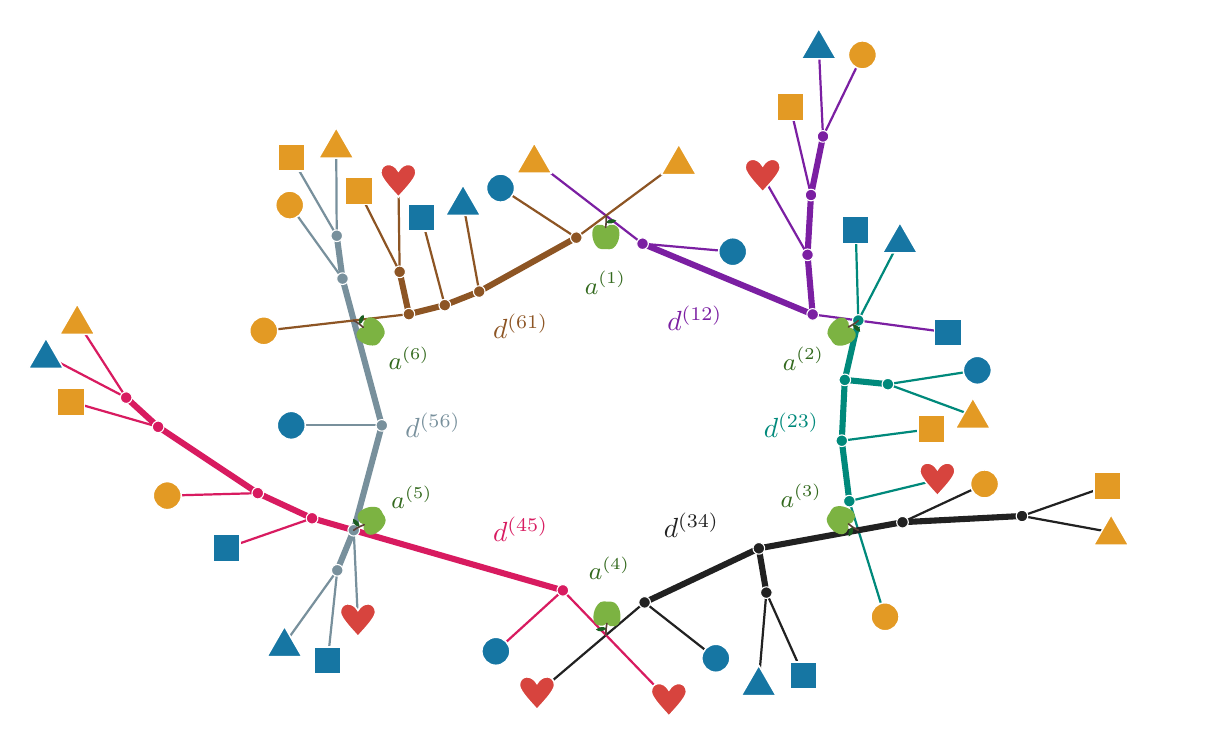
\begin{tikzpicture}[x=1cm,y=1cm]
% p^(12)
\draw[hex pendant,draw=hexTree1] (1.6092,2.2056)--(0.4637,2.3073);
\draw[hex pendant,draw=hexTree1] (2.7019,4.8183)--(2.7556,3.6696);
\draw[hex pendant,draw=hexTree1] (4.3443,1.1805)--(3.2043,1.3320);
\draw[hex pendant,draw=hexTree1] (2.3410,4.0447)--(2.6032,2.9250);
\draw[hex pendant,draw=hexTree1] (-0.9115,3.3652)--(0.0000,2.6640);
\draw[hex pendant,draw=hexTree1] (3.2565,4.7047)--(2.7556,3.6696);
\draw[hex internal,draw=hexTree1] (0.4637,2.3073)--(2.6244,1.4091);
\draw[hex pendant,draw=hexTree1] (0.4637,2.3073)--(0.0000,2.6640);
\draw[hex pendant,draw=hexTree1] (1.9897,3.1654)--(2.5591,2.1663);
\draw[hex internal,draw=hexTree1] (2.7556,3.6696)--(2.6032,2.9250);
\draw[hex internal,draw=hexTree1] (2.6032,2.9250)--(2.5591,2.1663);
\draw[hex internal,draw=hexTree1] (2.6244,1.4091)--(2.5591,2.1663);
\draw[hex pendant,draw=hexTree1] (2.6244,1.4091)--(3.2043,1.3320);
\node[hex vertex,fill=hexTree1] at (0.4637,2.3073) {};
\node[hex vertex,fill=hexTree1] at (2.7556,3.6696) {};
\node[hex vertex,fill=hexTree1] at (2.6032,2.9250) {};
\node[hex vertex,fill=hexTree1] at (2.5591,2.1663) {};
\node[hex vertex,fill=hexTree1] at (2.6244,1.4091) {};
\coordinate (v1) at (4.3443,1.1805);
\node[g2tree dark,rectangle,minimum size=3.4155000000000006mm,font={\sffamily\fontsize{6.6}{6.6}\selectfont\bfseries}] at (v1) {};
\coordinate (v2) at (2.7019,4.8183);
\begin{scope}[shift={(v2)},scale=0.7425000000000002,transform shape]
\path[fill=g2TaxonBlue,draw=white,line width=.55pt,line join=round] (0mm,3.0mm)--(-3.0mm,-2.2mm)--(3.0mm,-2.2mm)--cycle;
\end{scope}
\coordinate (v3) at (1.6092,2.2056);
\node[g2tree dark,circle,minimum size=3.5640000000000005mm,font={\sffamily\fontsize{6.6}{6.6}\selectfont\bfseries}] at (v3) {};
\coordinate (v4) at (2.3410,4.0447);
\node[g2tree light,rectangle,minimum size=3.4155000000000006mm,font={\sffamily\fontsize{6.6}{6.6}\selectfont\bfseries}] at (v4) {};
\coordinate (v5) at (-0.9115,3.3652);
\begin{scope}[shift={(v5)},scale=0.7425000000000002,transform shape]
\path[fill=g2TaxonYellow,draw=white,line width=.55pt,line join=round] (0mm,3.0mm)--(-3.0mm,-2.2mm)--(3.0mm,-2.2mm)--cycle;
\end{scope}
\coordinate (v6) at (3.2565,4.7047);
\node[g2tree light,circle,minimum size=3.5640000000000005mm,font={\sffamily\fontsize{6.6}{6.6}\selectfont\bfseries}] at (v6) {};
\coordinate (v7) at (1.9897,3.1654);
\begin{scope}[shift={(v7)},scale=0.7425000000000002,transform shape]
\path[fill=g2HeartRed,draw=white,line width=.55pt]
  (0mm,-2.7mm)..controls(-.45mm,-2.1mm)and(-3.0mm,.35mm)..(-3.0mm,1.45mm)
  ..controls(-3.0mm,3.2mm)and(-.9mm,3.4mm)..(0mm,1.75mm)
  ..controls(.9mm,3.4mm)and(3.0mm,3.2mm)..(3.0mm,1.45mm)
  ..controls(3.0mm,.35mm)and(.45mm,-2.1mm)..(0mm,-2.7mm)--cycle;
\end{scope}
% p^(23)
\draw[hex pendant,draw=hexTree2] (4.7160,0.6990)--(3.5796,0.5231);
\draw[hex pendant,draw=hexTree2] (3.7326,2.3535)--(3.2043,1.3320);
\draw[hex pendant,draw=hexTree2] (3.1711,2.4815)--(3.2043,1.3320);
\draw[hex pendant,draw=hexTree2] (4.1342,-0.0460)--(2.9939,-0.1949);
\draw[hex pendant,draw=hexTree2] (4.6588,0.1260)--(3.5796,0.5231);
\draw[hex pendant,draw=hexTree2] (3.5435,-2.4308)--(3.2043,-1.3320);
\draw[hex internal,draw=hexTree2] (3.0902,-0.9624)--(2.9939,-0.1949);
\draw[hex pendant,draw=hexTree2] (3.0902,-0.9624)--(3.2043,-1.3320);
\draw[hex pendant,draw=hexTree2] (4.2081,-0.6923)--(3.0902,-0.9624);
\draw[hex internal,draw=hexTree2] (3.5796,0.5231)--(3.0323,0.5778);
\draw[hex internal,draw=hexTree2] (2.9939,-0.1949)--(3.0323,0.5778);
\draw[hex internal,draw=hexTree2] (3.2043,1.3320)--(3.0323,0.5778);
\node[hex vertex,fill=hexTree2] at (3.0902,-0.9624) {};
\node[hex vertex,fill=hexTree2] at (3.5796,0.5231) {};
\node[hex vertex,fill=hexTree2] at (2.9939,-0.1949) {};
\node[hex vertex,fill=hexTree2] at (3.0323,0.5778) {};
\node[hex vertex,fill=hexTree2] at (3.2043,1.3320) {};
\coordinate (v1) at (3.1711,2.4815);
\node[g2tree dark,rectangle,minimum size=3.4155000000000006mm,font={\sffamily\fontsize{6.6}{6.6}\selectfont\bfseries}] at (v1) {};
\coordinate (v2) at (3.7326,2.3535);
\begin{scope}[shift={(v2)},scale=0.7425000000000002,transform shape]
\path[fill=g2TaxonBlue,draw=white,line width=.55pt,line join=round] (0mm,3.0mm)--(-3.0mm,-2.2mm)--(3.0mm,-2.2mm)--cycle;
\end{scope}
\coordinate (v3) at (4.7160,0.6990);
\node[g2tree dark,circle,minimum size=3.5640000000000005mm,font={\sffamily\fontsize{6.6}{6.6}\selectfont\bfseries}] at (v3) {};
\coordinate (v4) at (4.1342,-0.0460);
\node[g2tree light,rectangle,minimum size=3.4155000000000006mm,font={\sffamily\fontsize{6.6}{6.6}\selectfont\bfseries}] at (v4) {};
\coordinate (v5) at (4.6588,0.1260);
\begin{scope}[shift={(v5)},scale=0.7425000000000002,transform shape]
\path[fill=g2TaxonYellow,draw=white,line width=.55pt,line join=round] (0mm,3.0mm)--(-3.0mm,-2.2mm)--(3.0mm,-2.2mm)--cycle;
\end{scope}
\coordinate (v6) at (3.5435,-2.4308);
\node[g2tree light,circle,minimum size=3.5640000000000005mm,font={\sffamily\fontsize{6.6}{6.6}\selectfont\bfseries}] at (v6) {};
\coordinate (v7) at (4.2081,-0.6923);
\begin{scope}[shift={(v7)},scale=0.7425000000000002,transform shape]
\path[fill=g2HeartRed,draw=white,line width=.55pt]
  (0mm,-2.7mm)..controls(-.45mm,-2.1mm)and(-3.0mm,.35mm)..(-3.0mm,1.45mm)
  ..controls(-3.0mm,3.2mm)and(-.9mm,3.4mm)..(0mm,1.75mm)
  ..controls(.9mm,3.4mm)and(3.0mm,3.2mm)..(3.0mm,1.45mm)
  ..controls(3.0mm,.35mm)and(.45mm,-2.1mm)..(0mm,-2.7mm)--cycle;
\end{scope}
% p^(34)
\draw[hex pendant,draw=hexTree3] (1.3947,-2.9580)--(0.4896,-2.2485);
\draw[hex pendant,draw=hexTree3] (1.9387,-3.2698)--(2.0362,-2.1240);
\draw[hex pendant,draw=hexTree3] (2.5064,-3.1734)--(2.0362,-2.1240);
\draw[hex pendant,draw=hexTree3] (6.3683,-0.7704)--(5.2830,-1.1508);
\draw[hex pendant,draw=hexTree3] (6.4143,-1.3574)--(5.2830,-1.1508);
\draw[hex pendant,draw=hexTree3] (4.8075,-0.7442)--(3.7651,-1.2299);
\draw[hex internal,draw=hexTree3] (5.2830,-1.1508)--(3.7651,-1.2299);
\draw[hex pendant,draw=hexTree3] (-0.8768,-3.4081)--(0.0000,-2.6640);
\draw[hex internal,draw=hexTree3] (0.4896,-2.2485)--(1.9408,-1.5620);
\draw[hex pendant,draw=hexTree3] (0.4896,-2.2485)--(0.0000,-2.6640);
\draw[hex internal,draw=hexTree3] (1.9408,-1.5620)--(3.2043,-1.3320);
\draw[hex internal,draw=hexTree3] (2.0362,-2.1240)--(1.9408,-1.5620);
\draw[hex internal,draw=hexTree3] (3.7651,-1.2299)--(3.2043,-1.3320);
\node[hex vertex,fill=hexTree3] at (5.2830,-1.1508) {};
\node[hex vertex,fill=hexTree3] at (0.4896,-2.2485) {};
\node[hex vertex,fill=hexTree3] at (2.0362,-2.1240) {};
\node[hex vertex,fill=hexTree3] at (1.9408,-1.5620) {};
\node[hex vertex,fill=hexTree3] at (3.7651,-1.2299) {};
\coordinate (v1) at (2.5064,-3.1734);
\node[g2tree dark,rectangle,minimum size=3.4155000000000006mm,font={\sffamily\fontsize{6.6}{6.6}\selectfont\bfseries}] at (v1) {};
\coordinate (v2) at (1.9387,-3.2698);
\begin{scope}[shift={(v2)},scale=0.7425000000000002,transform shape]
\path[fill=g2TaxonBlue,draw=white,line width=.55pt,line join=round] (0mm,3.0mm)--(-3.0mm,-2.2mm)--(3.0mm,-2.2mm)--cycle;
\end{scope}
\coordinate (v3) at (1.3947,-2.9580);
\node[g2tree dark,circle,minimum size=3.5640000000000005mm,font={\sffamily\fontsize{6.6}{6.6}\selectfont\bfseries}] at (v3) {};
\coordinate (v4) at (6.3683,-0.7704);
\node[g2tree light,rectangle,minimum size=3.4155000000000006mm,font={\sffamily\fontsize{6.6}{6.6}\selectfont\bfseries}] at (v4) {};
\coordinate (v5) at (6.4143,-1.3574);
\begin{scope}[shift={(v5)},scale=0.7425000000000002,transform shape]
\path[fill=g2TaxonYellow,draw=white,line width=.55pt,line join=round] (0mm,3.0mm)--(-3.0mm,-2.2mm)--(3.0mm,-2.2mm)--cycle;
\end{scope}
\coordinate (v6) at (4.8075,-0.7442);
\node[g2tree light,circle,minimum size=3.5640000000000005mm,font={\sffamily\fontsize{6.6}{6.6}\selectfont\bfseries}] at (v6) {};
\coordinate (v7) at (-0.8768,-3.4081);
\begin{scope}[shift={(v7)},scale=0.7425000000000002,transform shape]
\path[fill=g2HeartRed,draw=white,line width=.55pt]
  (0mm,-2.7mm)..controls(-.45mm,-2.1mm)and(-3.0mm,.35mm)..(-3.0mm,1.45mm)
  ..controls(-3.0mm,3.2mm)and(-.9mm,3.4mm)..(0mm,1.75mm)
  ..controls(.9mm,3.4mm)and(3.0mm,3.2mm)..(3.0mm,1.45mm)
  ..controls(3.0mm,.35mm)and(.45mm,-2.1mm)..(0mm,-2.7mm)--cycle;
\end{scope}
% p^(45)
\draw[hex pendant,draw=hexTree4] (-1.3988,-2.8695)--(-0.5481,-2.0956);
\draw[hex pendant,draw=hexTree4] (-7.1127,0.8859)--(-6.0939,0.3524);
\draw[hex pendant,draw=hexTree4] (-4.8192,-1.5575)--(-3.7329,-1.1800);
\draw[hex pendant,draw=hexTree4] (-6.7933,0.2990)--(-5.6880,-0.0188);
\draw[hex pendant,draw=hexTree4] (-6.7162,1.3195)--(-6.0939,0.3524);
\draw[hex pendant,draw=hexTree4] (-5.5722,-0.8921)--(-4.4226,-0.8608);
\draw[hex pendant,draw=hexTree4] (-0.5481,-2.0956)--(0.0000,-2.6640);
\draw[hex internal,draw=hexTree4] (-0.5481,-2.0956)--(-3.2043,-1.3320);
\draw[hex pendant,draw=hexTree4] (0.7983,-3.4918)--(0.0000,-2.6640);
\draw[hex internal,draw=hexTree4] (-4.4226,-0.8608)--(-5.6880,-0.0188);
\draw[hex internal,draw=hexTree4] (-6.0939,0.3524)--(-5.6880,-0.0188);
\draw[hex internal,draw=hexTree4] (-3.7329,-1.1800)--(-4.4226,-0.8608);
\draw[hex internal,draw=hexTree4] (-3.7329,-1.1800)--(-3.2043,-1.3320);
\node[hex vertex,fill=hexTree4] at (-0.5481,-2.0956) {};
\node[hex vertex,fill=hexTree4] at (-4.4226,-0.8608) {};
\node[hex vertex,fill=hexTree4] at (-6.0939,0.3524) {};
\node[hex vertex,fill=hexTree4] at (-5.6880,-0.0188) {};
\node[hex vertex,fill=hexTree4] at (-3.7329,-1.1800) {};
\coordinate (v1) at (-4.8192,-1.5575);
\node[g2tree dark,rectangle,minimum size=3.4155000000000006mm,font={\sffamily\fontsize{6.6}{6.6}\selectfont\bfseries}] at (v1) {};
\coordinate (v2) at (-7.1127,0.8859);
\begin{scope}[shift={(v2)},scale=0.7425000000000002,transform shape]
\path[fill=g2TaxonBlue,draw=white,line width=.55pt,line join=round] (0mm,3.0mm)--(-3.0mm,-2.2mm)--(3.0mm,-2.2mm)--cycle;
\end{scope}
\coordinate (v3) at (-1.3988,-2.8695);
\node[g2tree dark,circle,minimum size=3.5640000000000005mm,font={\sffamily\fontsize{6.6}{6.6}\selectfont\bfseries}] at (v3) {};
\coordinate (v4) at (-6.7933,0.2990);
\node[g2tree light,rectangle,minimum size=3.4155000000000006mm,font={\sffamily\fontsize{6.6}{6.6}\selectfont\bfseries}] at (v4) {};
\coordinate (v5) at (-6.7162,1.3195);
\begin{scope}[shift={(v5)},scale=0.7425000000000002,transform shape]
\path[fill=g2TaxonYellow,draw=white,line width=.55pt,line join=round] (0mm,3.0mm)--(-3.0mm,-2.2mm)--(3.0mm,-2.2mm)--cycle;
\end{scope}
\coordinate (v6) at (-5.5722,-0.8921);
\node[g2tree light,circle,minimum size=3.5640000000000005mm,font={\sffamily\fontsize{6.6}{6.6}\selectfont\bfseries}] at (v6) {};
\coordinate (v7) at (0.7983,-3.4918);
\begin{scope}[shift={(v7)},scale=0.7425000000000002,transform shape]
\path[fill=g2HeartRed,draw=white,line width=.55pt]
  (0mm,-2.7mm)..controls(-.45mm,-2.1mm)and(-3.0mm,.35mm)..(-3.0mm,1.45mm)
  ..controls(-3.0mm,3.2mm)and(-.9mm,3.4mm)..(0mm,1.75mm)
  ..controls(.9mm,3.4mm)and(3.0mm,3.2mm)..(3.0mm,1.45mm)
  ..controls(3.0mm,.35mm)and(.45mm,-2.1mm)..(0mm,-2.7mm)--cycle;
\end{scope}
% p^(56)
\draw[hex pendant,draw=hexTree5] (-3.9974,0.0000)--(-2.8474,0.0000);
\draw[hex pendant,draw=hexTree5] (-4.0838,-2.7750)--(-3.4133,-1.8407);
\draw[hex pendant,draw=hexTree5] (-3.5335,-2.9844)--(-3.4133,-1.8407);
\draw[hex pendant,draw=hexTree5] (-3.9950,3.4043)--(-3.4200,2.4083);
\draw[hex pendant,draw=hexTree5] (-3.4267,3.5583)--(-3.4200,2.4083);
\draw[hex pendant,draw=hexTree5] (-4.0172,2.7975)--(-3.3466,1.8633);
\draw[hex internal,draw=hexTree5] (-3.4200,2.4083)--(-3.3466,1.8633);
\draw[hex pendant,draw=hexTree5] (-3.1508,-2.4808)--(-3.2043,-1.3320);
\draw[hex internal,draw=hexTree5] (-2.8474,0.0000)--(-3.2043,-1.3320);
\draw[hex internal,draw=hexTree5] (-2.8474,0.0000)--(-3.2043,1.3320);
\draw[hex internal,draw=hexTree5] (-3.4133,-1.8407)--(-3.2043,-1.3320);
\draw[hex internal,draw=hexTree5] (-3.3466,1.8633)--(-3.2043,1.3320);
\node[hex vertex,fill=hexTree5] at (-3.4200,2.4083) {};
\node[hex vertex,fill=hexTree5] at (-2.8474,0.0000) {};
\node[hex vertex,fill=hexTree5] at (-3.4133,-1.8407) {};
\node[hex vertex,fill=hexTree5] at (-3.2043,-1.3320) {};
\node[hex vertex,fill=hexTree5] at (-3.3466,1.8633) {};
\coordinate (v1) at (-3.5335,-2.9844);
\node[g2tree dark,rectangle,minimum size=3.4155000000000006mm,font={\sffamily\fontsize{6.6}{6.6}\selectfont\bfseries}] at (v1) {};
\coordinate (v2) at (-4.0838,-2.7750);
\begin{scope}[shift={(v2)},scale=0.7425000000000002,transform shape]
\path[fill=g2TaxonBlue,draw=white,line width=.55pt,line join=round] (0mm,3.0mm)--(-3.0mm,-2.2mm)--(3.0mm,-2.2mm)--cycle;
\end{scope}
\coordinate (v3) at (-3.9974,0.0000);
\node[g2tree dark,circle,minimum size=3.5640000000000005mm,font={\sffamily\fontsize{6.6}{6.6}\selectfont\bfseries}] at (v3) {};
\coordinate (v4) at (-3.9950,3.4043);
\node[g2tree light,rectangle,minimum size=3.4155000000000006mm,font={\sffamily\fontsize{6.6}{6.6}\selectfont\bfseries}] at (v4) {};
\coordinate (v5) at (-3.4267,3.5583);
\begin{scope}[shift={(v5)},scale=0.7425000000000002,transform shape]
\path[fill=g2TaxonYellow,draw=white,line width=.55pt,line join=round] (0mm,3.0mm)--(-3.0mm,-2.2mm)--(3.0mm,-2.2mm)--cycle;
\end{scope}
\coordinate (v6) at (-4.0172,2.7975);
\node[g2tree light,circle,minimum size=3.5640000000000005mm,font={\sffamily\fontsize{6.6}{6.6}\selectfont\bfseries}] at (v6) {};
\coordinate (v7) at (-3.1508,-2.4808);
\begin{scope}[shift={(v7)},scale=0.7425000000000002,transform shape]
\path[fill=g2HeartRed,draw=white,line width=.55pt]
  (0mm,-2.7mm)..controls(-.45mm,-2.1mm)and(-3.0mm,.35mm)..(-3.0mm,1.45mm)
  ..controls(-3.0mm,3.2mm)and(-.9mm,3.4mm)..(0mm,1.75mm)
  ..controls(.9mm,3.4mm)and(3.0mm,3.2mm)..(3.0mm,1.45mm)
  ..controls(3.0mm,.35mm)and(.45mm,-2.1mm)..(0mm,-2.7mm)--cycle;
\end{scope}
% p^(61)
\draw[hex pendant,draw=hexTree6] (-1.3399,3.0137)--(-0.3776,2.3840);
\draw[hex pendant,draw=hexTree6] (-1.8161,2.8307)--(-1.6105,1.6992);
\draw[hex pendant,draw=hexTree6] (-2.3415,2.6384)--(-2.0477,1.5266);
\draw[hex pendant,draw=hexTree6] (-3.1394,2.9763)--(-2.6209,1.9498);
\draw[hex pendant,draw=hexTree6] (0.9238,3.3489)--(0.0000,2.6640);
\draw[hex pendant,draw=hexTree6] (-4.3468,1.2008)--(-3.2043,1.3320);
\draw[hex internal,draw=hexTree6] (-0.3776,2.3840)--(-1.6105,1.6992);
\draw[hex pendant,draw=hexTree6] (-0.3776,2.3840)--(0.0000,2.6640);
\draw[hex pendant,draw=hexTree6] (-2.6370,3.0997)--(-2.6209,1.9498);
\draw[hex internal,draw=hexTree6] (-2.0477,1.5266)--(-2.5038,1.4124);
\draw[hex pendant,draw=hexTree6] (-2.5038,1.4124)--(-3.2043,1.3320);
\draw[hex internal,draw=hexTree6] (-2.6209,1.9498)--(-2.5038,1.4124);
\draw[hex internal,draw=hexTree6] (-1.6105,1.6992)--(-2.0477,1.5266);
\node[hex vertex,fill=hexTree6] at (-0.3776,2.3840) {};
\node[hex vertex,fill=hexTree6] at (-2.0477,1.5266) {};
\node[hex vertex,fill=hexTree6] at (-2.6209,1.9498) {};
\node[hex vertex,fill=hexTree6] at (-2.5038,1.4124) {};
\node[hex vertex,fill=hexTree6] at (-1.6105,1.6992) {};
\coordinate (v1) at (-2.3415,2.6384);
\node[g2tree dark,rectangle,minimum size=3.4155000000000006mm,font={\sffamily\fontsize{6.6}{6.6}\selectfont\bfseries}] at (v1) {};
\coordinate (v2) at (-1.8161,2.8307);
\begin{scope}[shift={(v2)},scale=0.7425000000000002,transform shape]
\path[fill=g2TaxonBlue,draw=white,line width=.55pt,line join=round] (0mm,3.0mm)--(-3.0mm,-2.2mm)--(3.0mm,-2.2mm)--cycle;
\end{scope}
\coordinate (v3) at (-1.3399,3.0137);
\node[g2tree dark,circle,minimum size=3.5640000000000005mm,font={\sffamily\fontsize{6.6}{6.6}\selectfont\bfseries}] at (v3) {};
\coordinate (v4) at (-3.1394,2.9763);
\node[g2tree light,rectangle,minimum size=3.4155000000000006mm,font={\sffamily\fontsize{6.6}{6.6}\selectfont\bfseries}] at (v4) {};
\coordinate (v5) at (0.9238,3.3489);
\begin{scope}[shift={(v5)},scale=0.7425000000000002,transform shape]
\path[fill=g2TaxonYellow,draw=white,line width=.55pt,line join=round] (0mm,3.0mm)--(-3.0mm,-2.2mm)--(3.0mm,-2.2mm)--cycle;
\end{scope}
\coordinate (v6) at (-4.3468,1.2008);
\node[g2tree light,circle,minimum size=3.5640000000000005mm,font={\sffamily\fontsize{6.6}{6.6}\selectfont\bfseries}] at (v6) {};
\coordinate (v7) at (-2.6370,3.0997);
\begin{scope}[shift={(v7)},scale=0.7425000000000002,transform shape]
\path[fill=g2HeartRed,draw=white,line width=.55pt]
  (0mm,-2.7mm)..controls(-.45mm,-2.1mm)and(-3.0mm,.35mm)..(-3.0mm,1.45mm)
  ..controls(-3.0mm,3.2mm)and(-.9mm,3.4mm)..(0mm,1.75mm)
  ..controls(.9mm,3.4mm)and(3.0mm,3.2mm)..(3.0mm,1.45mm)
  ..controls(3.0mm,.35mm)and(.45mm,-2.1mm)..(0mm,-2.7mm)--cycle;
\end{scope}
\pic[rotate=-0.5,scale=0.750] at (0.0000,2.6640) {g2apple};
\node[hex point label] at (-0.0076,1.8140) {\(a^{(1)}\)};
\node[hex line label,text=hexTree1] at (1.1286,1.3583) {\(d^{(12)}\)};
\pic[rotate=-55.2,scale=0.750] at (3.2043,1.3320) {g2apple};
\node[hex point label] at (2.5062,0.8470) {\(a^{(2)}\)};
\node[hex line label,text=hexTree2] at (2.3535,-0.0013) {\(d^{(23)}\)};
\pic[rotate=238.7,scale=0.750] at (3.2043,-1.3320) {g2apple};
\node[hex point label] at (2.4777,-0.8909) {\(a^{(3)}\)};
\node[hex line label,text=hexTree3] at (1.0840,-1.2731) {\(d^{(34)}\)};
\pic[rotate=177.1,scale=0.750] at (0.0000,-2.6640) {g2apple};
\node[hex point label] at (0.0424,-1.8151) {\(a^{(4)}\)};
\node[hex line label,text=hexTree4] at (-1.0843,-1.3205) {\(d^{(45)}\)};
\pic[rotate=119.5,scale=0.750] at (-3.2043,-1.3320) {g2apple};
\node[hex point label] at (-2.4643,-0.9137) {\(a^{(5)}\)};
\node[hex line label,text=hexTree5] at (-2.1974,0.0000) {\(d^{(56)}\)};
\pic[rotate=55.8,scale=0.750] at (-3.2043,1.3320) {g2apple};
\node[hex point label] at (-2.5015,0.8539) {\(a^{(6)}\)};
\node[hex line label,text=hexTree6] at (-1.0844,1.2631) {\(d^{(61)}\)};
% Center the hexagon of apples, whose center is the origin, on the page: extend the bounding box
% symmetrically about x=0, so that \centering in main.tex centers the origin and not the pendant edges.
\newdimen\hexbbwest \newdimen\hexbbeast
\pgfextractx{\hexbbwest}{\pgfpointanchor{current bounding box}{west}}
\pgfextractx{\hexbbeast}{\pgfpointanchor{current bounding box}{east}}
\path (-\hexbbeast,0cm) -- (-\hexbbwest,0cm);
\end{tikzpicture}
\endgroup
